\section{Introduction}
 

Throughout the design process it is assumed that the controller output signal corresponds linearly to the voltage at the motor terminals.
%
An amplifier circuit transforms the low-power DAC output signal to a signal capable of controlling the motor using a PWM power amplifier.
As a subsystem, the desired amplifier response should be linear as shown in figure \ref{fig:iodesired}.
In the figure, amplifier gain is assumed to be one; any amplifier gain can be modeled external to the compensator block at a later time.
The amplifier does not naturally % Change naturally
have the response shown in figure \ref{fig:iodesired} and as such new compensator subsystem is needed to account for amplifier non-linearities.
This compensator must account for two system characteristics.
%
First, the amplifiers gain, offset and dead zone.
Second, motor back EMF and the fact % change "the fact"
the amplifier is not a voltage amplifier but an open loop power amplifier.
The observed amplifier transfer function is similar to that shown in figure \ref{fig:ioactual}.


%Desired response
\begin{figure}[ht]
    \centering
    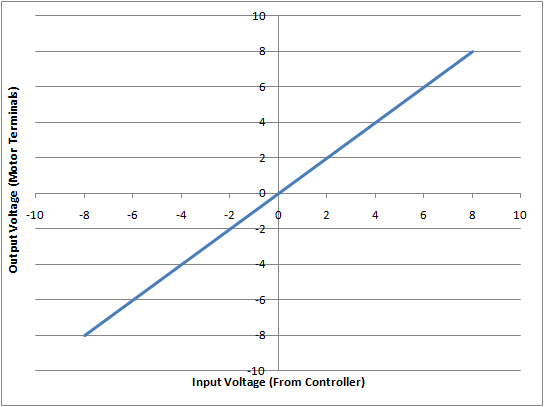
\includegraphics[width=.60\textwidth]{images/InputVsOutputDesired.png}
    \caption{Desired Amplifier Transfer Function}
    \label{fig:iodesired}
\end{figure}

\begin{figure}[ht]
    \centering
    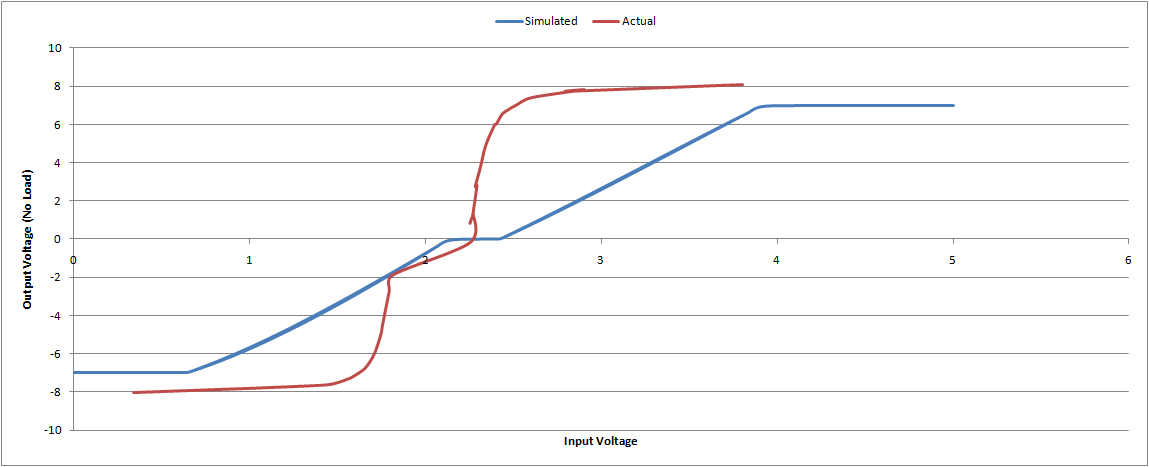
\includegraphics[width=.95\textwidth]{images/OutputVoltage.png}
    \caption{Observed Characteristics with Motor Load}
    \label{fig:ioactual}
\end{figure}